\begin{figure}[h]
    \centering
    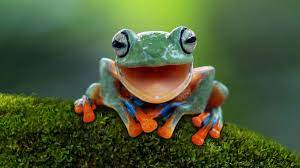
\includegraphics{download.jpeg}
    \caption{Example}
    \label{fig:results}
\end{figure}

Look at Figure~\ref{fig:results} for an example.

If~\cite{caselloTransportationActivityCenters2006} we want a page with no headers or footers except for a simple page number at the bottom we would use the keyword plain. However you need to be aware that using this command changes the page style for all the pages following the command. Therefore we need to turn the page style back to fancy as soon as we want the headers back.

If~\citep{caselloTransportationActivityCenters2006} we want a page with no headers or footers except for a simple page number at the bottom we would use the keyword plain. However you need to be aware that using this command changes the page style for all the pages following the command. Therefore we need to turn the page style back to fancy as soon as we want the headers back.

If~\citet{caselloTransportationActivityCenters2006} we want a page with no headers or footers except for a simple page number at the bottom we would use the keyword plain. However you need to be aware that using this command changes the page style for all the pages following the command. Therefore we need to turn the page style back to fancy as soon as we want the headers back.

This concludes our discussion on page layout. In the next post we'll look at using images and tables.If we want a page with no headers or footers except for a simple page number at the bottom we would use the keyword plain. However you need to be aware that using this command changes the page style for all the pages following the command. Therefore we need to turn the page style back to fancy as soon as we want the headers back.

This concludes our discussion on page layout. In the next post we'll look at using images and tables.If we want a page with no headers or footers except for a simple page number at the bottom we would use the keyword plain. However you need to be aware that using this command changes the page style for all the pages following the command. Therefore we need to turn the page style back to fancy as soon as we want the headers back.

This concludes our discussion on page layout. In the next post we'll look at using images and tables.If we want a page with no headers or footers except for a simple page number at the bottom we would use the keyword plain. However you need to be aware that using this command changes the page style for all the pages following the command. Therefore we need to turn the page style back to fancy as soon as we want the headers back.

This concludes our discussion on page layout. In the next post we'll look at using images and tables.If we want a page with no headers or footers except for a simple page number at the bottom we would use the keyword plain. However you need to be aware that using this command changes the page style for all the pages following the command. Therefore we need to turn the page style back to fancy as soon as we want the headers back.

This concludes our discussion on page layout. In the next post we'll look at using images and tables.If we want a page with no headers or footers except for a simple page number at the bottom we would use the keyword plain. However you need to be aware that using this command changes the page style for all the pages following the command. Therefore we need to turn the page style back to fancy as soon as we want the headers back.

This concludes our discussion on page layout. In the next post we'll look at using images and tables.If we want a page with no headers or footers except for a simple page number at the bottom we would use the keyword plain. However you need to be aware that using this command changes the page style for all the pages following the command. Therefore we need to turn the page style back to fancy as soon as we want the headers back.

This concludes our discussion on page layout. In the next post we'll look at using images and tables.If we want a page with no headers or footers except for a simple page number at the bottom we would use the keyword plain. However you need to be aware that using this command changes the page style for all the pages following the command. Therefore we need to turn the page style back to fancy as soon as we want the headers back.

This concludes our discussion on page layout. In the next post we'll look at using images and tables.If we want a page with no headers or footers except for a simple page number at the bottom we would use the keyword plain. However you need to be aware that using this command changes the page style for all the pages following the command. Therefore we need to turn the page style back to fancy as soon as we want the headers back.

This concludes our discussion on page layout. In the next post we'll look at using images and tables.If we want a page with no headers or footers except for a simple page number at the bottom we would use the keyword plain. However you need to be aware that using this command changes the page style for all the pages following the command. Therefore we need to turn the page style back to fancy as soon as we want the headers back.

This concludes our discussion on page layout. In the next post we'll look at using images and tables.If we want a page with no headers or footers except for a simple page number at the bottom we would use the keyword plain. However you need to be aware that using this command changes the page style for all the pages following the command. Therefore we need to turn the page style back to fancy as soon as we want the headers back.

This concludes our discussion on page layout. In the next post we'll look at using images and tables.If we want a page with no headers or footers except for a simple page number at the bottom we would use the keyword plain. However you need to be aware that using this command changes the page style for all the pages following the command. Therefore we need to turn the page style back to fancy as soon as we want the headers back.

This concludes our discussion on page layout. In the next post we'll look at using images and tables.If we want a page with no headers or footers except for a simple page number at the bottom we would use the keyword plain. However you need to be aware that using this command changes the page style for all the pages following the command. Therefore we need to turn the page style back to fancy as soon as we want the headers back.

This concludes our discussion on page layout. In the next post we'll look at using images and tables.If we want a page with no headers or footers except for a simple page number at the bottom we would use the keyword plain. However you need to be aware that using this command changes the page style for all the pages following the command. Therefore we need to turn the page style back to fancy as soon as we want the headers back.

This concludes our discussion on page layout. In the next post we'll look at using images and tables.If we want a page with no headers or footers except for a simple page number at the bottom we would use the keyword plain. However you need to be aware that using this command changes the page style for all the pages following the command. Therefore we need to turn the page style back to fancy as soon as we want the headers back.

This concludes our discussion on page layout. In the next post we'll look at using images and tables.If we want a page with no headers or footers except for a simple page number at the bottom we would use the keyword plain. However you need to be aware that using this command changes the page style for all the pages following the command. Therefore we need to turn the page style back to fancy as soon as we want the headers back.

This concludes our discussion on page layout. In the next post we'll look at using images and tables.